\chapter{関連研究}
\label{related_works}

近年、道具や機械、VR上のアバター、そしてインタラクティブな作品といった対象と、人との関係を捉える言葉として、「embodiment」が用いられている。Embodimentの意味は「具現化、身体化」など様々だが、本章では「embodiment」を「身体化」として捉える立場、「一体化」として捉える立場について紹介する。その上で、本研究が着目する「人馬一体」について、「``一体化''としてのembodiment」の立場にあると考えられる、Sydney Felsの提唱したモデルを用いて説明し、本研究の位置付けを明らかにする。

\section{``身体化''としてのembodiment}
「身体化(embodiment)」は心理学や認知科学の領域で、「身体化感覚(sense of embodiment)」を中心として実証的知見が蓄積されている。身体化感覚は、身体に対する所有感(sense of body ownership)、行為主体感(sense of agency)、そして自己位置感覚(sense of self-location)を合わせた感覚として取り扱われることが多い\cite{kilteni2012}。その元となったのは、Gallagherの「ミニマルセルフ」という概念である。「ミニマルセルフ」とは、自我としてみなしうる必要最小限のもののことであり、身体所有感(sense of ownership)、行為主体感(sense of agency)の二つから構成されていると説明される\cite{Gallagher2000}。こうした自己についての説明を実験的に操作・検証可能であることを示したのがBotvinick \& Cohenによるラバーハンド錯覚\cite{BotvinickCohen1998}である。これは、自分の手を衝立の裏に隠し、ラバー製の手を目の前に置いた状態で、両方に同じタイミングで刺激を提示すると、偽物の手を自分の手であるように感じる錯覚である。この報告により、外界の対象への身体所有感の生起が可能であることが示されたとともに、身体所有感研究に関する系統的な手法が探求されることとなった。

VRやロボティクスなどの分野では、「私たちはどこまでを自分の身体として認識(身体化)しうるか?」について、その可能性と限界を探る研究や、そうした知見の応用を提唱する研究へと繋がっている。以下では、身体化感覚における探求や応用について、一例を紹介する。

VRを用いた身体化感覚の研究では、身体の別の部位への動きのマッピングやユーザが同時に操作する身体の数などを操作変数とすることで、新しい心理学研究の可能性を拓くような研究がなされている。例えば近藤ら\cite{Kondo2020}は、右手の親指の動きにVR上の左腕の動きを連動させることで錯覚的な身体所有感(Illusory Ownership)が生じるのかについて検証した。被験者は、右手の親指の動きがVR上での左腕の動きにマッピングされている様子をヘッドマウントディスプレイを介して確認する。実験では、被験者に5分間自由に指先を動かしてもらった後、VR上で左腕のあたりにナイフが突然出現する。このときの皮膚コンダクタンス反応(Skin Conductance Response, SCR)の計測と、身体化感覚(embodiment)に関するアンケートを20人の被験者に行った結果、この手法を通して右手の親指と左腕の結びつき(re-association)は、程度は弱いが誘発できると報告している。また三浦ら\cite{miura2022multisoma}は、VR上で最大4つの身体を制御できるシステムを実装し、複数の身体を制御する際、人間の身体認知がいかに更新されるかについて検討した。実験では3つのタスクを設定し、視線情報、タスクのパフォーマンス、身体化感覚(sense of embodiment)についての主観評価により、これらの身体の認知を評価した。結果、人間は複数の身体を同時に操作することで、それぞれの身体に対して身体所有感(sense of ownership)や運動主体感(sense of agency)を持つことができると報告している。

また、トレーニングを通した身体化感覚の変化を扱う研究も行われている。Kielibaら\cite{kieliba2021robotic}は、ロボットで拡張された親指が人間の運動能力を拡張させることができるかどうか、そしてそれが手の神経表現や機能にどのような影響を与えるのかを調査するため、The Third Thumbというロボットの親指を用いた研究を行った。この親指は、足のつま先で操作することができる。5人の参加者は、5日間にわたってThe Third Thumbを装着し、実験室での使用と日常生活での使用が求められた。通常は両手を使って行うタスクをこの親指を駆使して片手で行い、その器用さ(dexterity)や身体化感覚(sense of embodiment)などの度合いが評価された。トレーニングを経て、認知的負荷が増加した場合や視覚が遮断された場合でも、親指の運動制御、器用さ、そしてThe Third Thumbに対する身体化感覚(sense of embodiment)が向上したと報告している。

さらに、こうした考え方をユーザインターフェースのような道具の操作性について議論するために援用する例も見られる。インターフェース研究者の渡邊は、ユーザインターフェースにおける「透明性」を実現する上で「自己帰属感(sense of ownership)」に着目した\cite{Watanabe2017}。ここで「透明性」とは、道具の使用において、使っている最中にはその道具自体を意識せずに身体の一部になったかのようになり、目的に集中できるようにすることとされている。そして、道具の透明性は「自己帰属感」によってもたらされると考え、マウスカーソルを対象に、ユーザインターフェースにおける自己帰属感を検証する「ダミーカーソル実験」を行った\cite{Watanabe2013}。この実験ではスクリーン上に、マウスと連動して動く通常のカーソルの他に色形状の同じの複数のダミーのカーソルをランダムに動くように同時に提示する。被験者は動きのみでしか自身のカーソルを判別することができない環境になる。そしてこの実験によって、人は動きのみであっても複数のダミーカーソルの中から自身のカーソルを発見できると報告されている。どれが自分のカーソルか判別できることから、人間はカーソルに対しても自己を見出しており、自己帰属感が生起していると主張している。これを踏まえて、ユーザインターフェースにおける自己帰属感を生起するために、操作時の動作とグラフィックの追従性が重要となることを指摘した。

\section{``一体化''としてのembodiment}
ここまで概観したように、「``身体化''としてのembodiment」については、その探究や応用を提示する研究が発展してきた。しかし、これらの議論で前提とされてきた「自己に帰属する他者」という意味でのembodimentのみでは、捉えきれない人と対象との関係があるのではないだろうか。
ここで、embodimentという言葉について原義に立ち返って考えたい。Embodimentは日本語で「身体化、具体化」などと訳されるが、動詞の「embody」についてCambridge Dictionaryで引くと、
\begin{quote}
  \begin{enumerate}
    \item \textit{to represent a quality or an idea exactly} (質や考えを的確に表すこと) 
    \item \textit{to include as part of something} ((何かを)何かの一部として取り込むこと)
  \end{enumerate}
\end{quote}
とある\cite{embody}。ここで指摘したいのは、2つ目の意味からembodimentの原義とは「何かを取り込んで、何かの一部とすること」であり、「人間の一部として対象が帰属しているような状態」のみを指すわけではないということだ。「自己に帰属する他者」という主従関係(=身体化)から自由になって人と他者との関係を捉え直すと、embodimentの研究には「他者に帰属する自己」という関係も捉えられるようになる。このような、自己と他者の主従関係を問わないembodimentを、ここでは「``一体化''としてのembodiment」とする。本節では、そのような立場からembodimentを捉えていると考えられる研究を2つ紹介する。

\subsection{人馬一体感}
心理学研究者の大北らは、ヒトとウマという異種間の間に芽生える一体感である「人馬一体」感について、どのようなプロセスで生じるのか、またそれはどのような感覚なのかを明らかにする目的で、馬術経験者に対するインタビューから概念生成を行った\cite{ohkita2018}。結果、人がウマに対しておこなう「扶助」と呼ばれる非言語シグナルに対して、時間的に接近してウマが行動を変化させたときに、操作主体感といった自己の身体保持感(sense of ownership)の拡張が生じるだけでなく、ウマというヒト(自己)以外のエージェントが協働したことによって「ウマと心が通じ合えた」といった円滑なインタラクション感も得ている可能性が示されたと報告している。このように、自己と他者との関係について、一方的に人に帰属するような他者の観点のみならず、ヒトとウマの間に芽生えた相互学習や、ヒトが対象に対して帰属していくような感覚を通して、一体感が生起することを捉える視点も存在する。

\subsection{Sidney Felsによるembodiment}
コンピューター工学者のSidney Felsは、「Intimacy and Embodiment: Implications for Art and Technology」\cite{Fels}において、人間と対象との関係性を「embodiment」の観点から4つのカテゴリに分類した。このようなモデルを用いることで、Fels自身が制作したインタラクティブ作品である《Iamascope》をはじめ、複数の事例に関して人と対象との関係を説明する。《Iamascope》とは、ビデオカメラの前に立つ体験者の動きに応じて、映像と音が変化する万華鏡のような作品である。Felsは、人と対象との4つの関係のそれぞれで、異なる美的体験をしていると説明する。

その背景には、90年代に演算装置を用いた作品が登場し、鑑賞だけではない作品との関係が生じた中で、芸術表現に科学技術を用いることを特徴づけるものを捉えたいという意図があったと考えられる。Felsによる4つの分類は、その後もインタラクティブアートの研究において参照されている。例えばCostelloらは、Felsの《Iamascope》についての詳細な主観体験の言語データを、体験者自身が、作品体験時の映像を通して振り返るvideo-cued recallという手法を用いて収集し、《Iamascope》の体験の中で起こっていたことについての分析を、Felsの分類を用いて行った。

Felsが行った分類について、各カテゴリの説明は以下の通りである(これらのカテゴリ名はCostelloら\cite{Costello2005}による。括弧内は筆者訳)。

\textbf{\textit{Response}(応答):}\\
対象に働きかけ、その応答次第で何をするか決める「対話」のような対象との関係を指す。この時は、人と対象とのあいだに一体感は芽生えていない。Felsは、人と対象がこの関係下にあるときに感じる美的体験とは、人が期待していたことに対して予想通りの反応が得られるかどうかにかかっているという。Felsはこの関係下にある状態の例として「コンピュータとそれに初めて触れた人」を挙げ、「なんらかの操作を通して得られた、便利な機能に喜んでいる状態と説明する。

\textbf{\textit{Control}(制御):}\\
人は対象を、自分自身の延長のように感じている。このときに感じる感情的な満足や美的体験とは、操作そのものによってもたらされる。これは例えばピアノの演奏において、「音が出ている」ということだけでなく、自分自身の表現したいことが、不自由なくピアノを通して体現されていると感じるときの、一体感によってもたらされる心地よさが該当する \footnote{「Control」においてFelsは、「自分自身の延長」として経験される感覚であり、またそれが追従性の高いグラフィックによってもたらされると説明する。これは、渡邊がマウスカーソルやスマートフォンに対して用いた「操作時の指とグラフィックの追従性が高い」インターフェースという説明と同等のものであると考えられる。このことからFelsの分類におけるControlは、渡邊の「自己帰属感」と重なる。}。

\textbf{\textit{Contemplation}(熟考):}\\
人が対象からの信号やメッセージについて、内省や熟考することを通じて、感情的になったり美的体験を得る状態を指す。このとき、人が対象に対して働きかけることはない。その具体例として、絵画の鑑賞体験が該当する。

\textbf{\textit{Belonging}(帰属):}\\
対象によって人が動かされているような経験を指す。人はその対象によって提供される体験を通じて感情的な反応を得る。ここでは、対象が人の体験や感情を形作る役割を果たす。

\begin{figure}[H]
  \centering
  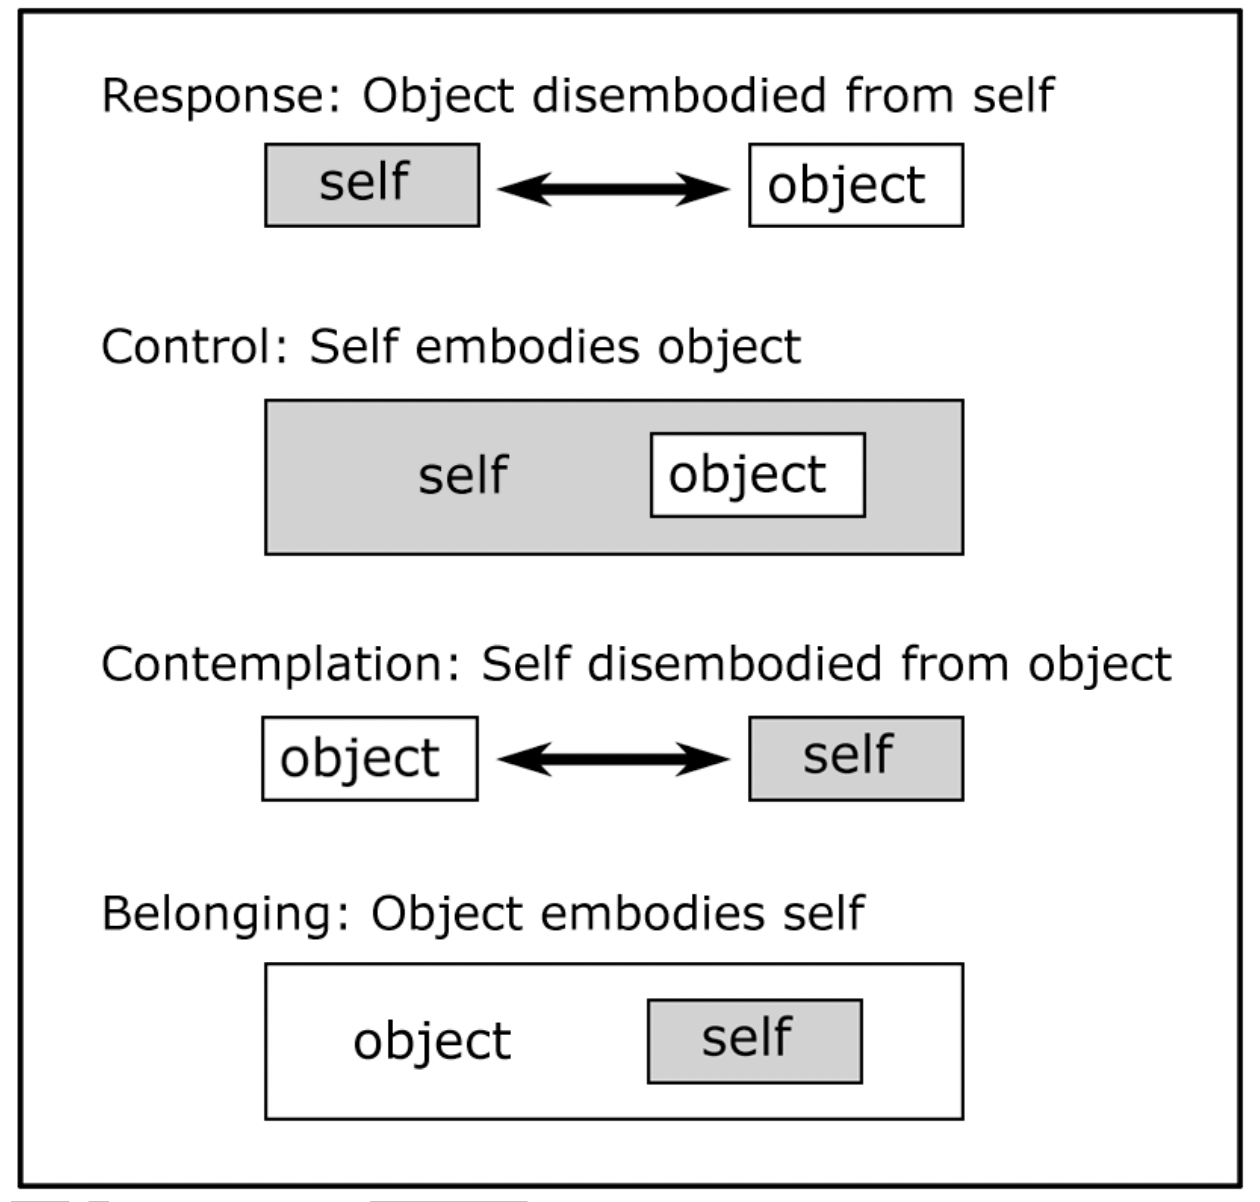
\includegraphics[width=8cm]{img/fels_diagram.png}
  \caption{Felsによるembodiment: Costelloらの論文より引用}
  \label{fig:fels_embodiment}
\end{figure}

本研究では、これら「``一体化''としてのembodiment」の立場から、自己と他者の双方向的な一体感が象徴的に現れる「人馬一体」という言葉に着目し、そうした関係性のデザインを目指す。ここでの「人馬一体」感とは、例えば楽器やバイクなどに無生物とのあいだにもみられるものであり、実現しようと思う自身の目的意識に対して自己と他者のあいだで折り合いをつけていくことで生じる一体化の感覚を指す。こうした一体化のプロセスを捉えるために、本研究ではFelsの分類を用いて、作品の体験について分析することとした。Felsの分類は、《Iamascope》のようなインタラクティブな作品と体験者との関係を説明するために考案されたモデルであり、本研究が取り組む手指の変換という表現における、作品と体験者との関係の変化を説明する際の手段として妥当である。これらの理由から、本研究では制作されたプロトタイプ、作品におけるねらい、そしてその結果について、Felsの分類に基づき分析することとした。